\documentclass{ip-lab}

\lablevel{n4}
\labnumber{Laboratorio 3}
\labtitle{Análisis de datos y matrices}

\makeheader

\begin{document}

\maketitle

\begin{sectionbox}{Preparación del ambiente de trabajo}
Para este laboratorio debe trabajar con dos módulos: \texttt{analisis\_musica.py} para las actividades de visualización y \texttt{matrices.py} para las actividades de matrices.

Se le proporcionará:
\begin{itemize}
    \item Un archivo \texttt{cupicharts.csv} con datos de canciones en las listas de popularidad.
    \item Un esqueleto del módulo \texttt{analisis\_musica.py} que ya incluye el código para cargar el CSV y toda la lógica de graficación. Su tarea es implementar únicamente la lógica de filtrado y transformación de datos con Pandas dentro de cada función; el código que genera las gráficas ya está incluido en el esqueleto.
\end{itemize}
\end{sectionbox}

\pagebreak

\begin{sectionbox}{Actividad 1: Canciones por género de un artista}

En el esqueleto de \texttt{analisis\_musica.py}, complete la función \texttt{canciones\_por\_genero\_artista}, que recibe el DataFrame y el nombre de un artista. Implemente la lógica de Pandas para:

\begin{itemize}
    \item Filtrar las filas del DataFrame para quedarse solo con las canciones del artista dado.
    \item Contar cuántas canciones tiene ese artista en cada género musical y guardar el resultado en la variable \texttt{conteo}.
\end{itemize}

El código del esqueleto usará su variable \texttt{conteo} para generar la siguiente gráfica:

\begin{center}
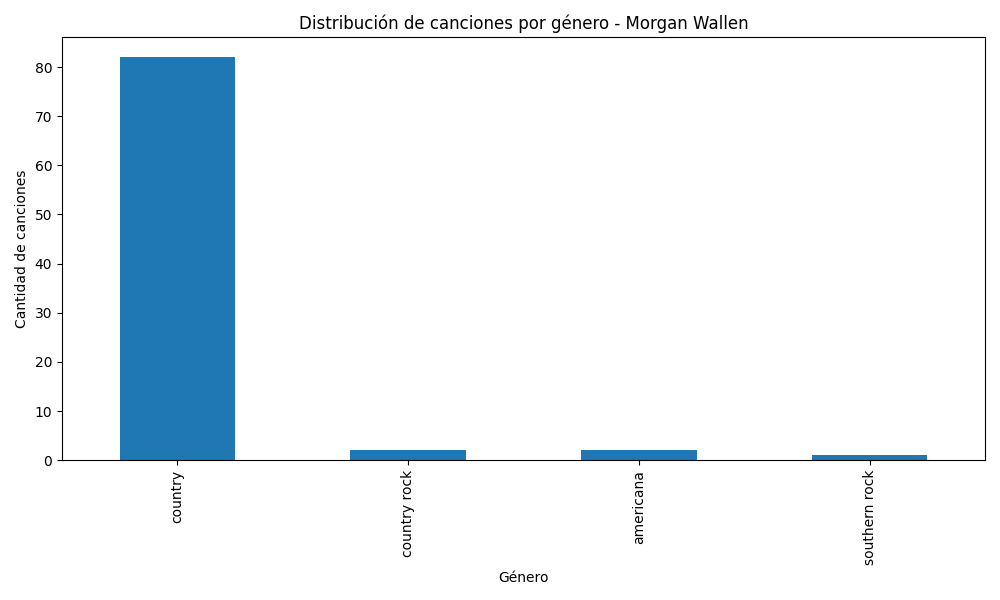
\includegraphics[width=0.7\textwidth]{by_genre.png}
\end{center}

\end{sectionbox}

\pagebreak

\begin{sectionbox}{Actividad 2: Popularidad total por género}

En el esqueleto de \texttt{analisis\_musica.py}, complete la función \texttt{popularidad\_por\_genero\_explicitidad}, que recibe el DataFrame y un valor booleano indicando si se quieren analizar canciones explícitas o no explícitas. Implemente la lógica de Pandas para:

\begin{itemize}
    \item Filtrar las canciones según si son explícitas o no.
    \item Agrupar por género y sumar la popularidad total de cada género.
    \item Ordenar de mayor a menor y quedarse solo con los 20 géneros más populares.
    \item Guardar el resultado en la variable \texttt{popularidad}.
\end{itemize}

El código del esqueleto usará su variable \texttt{popularidad} para generar la siguiente gráfica:

\begin{center}
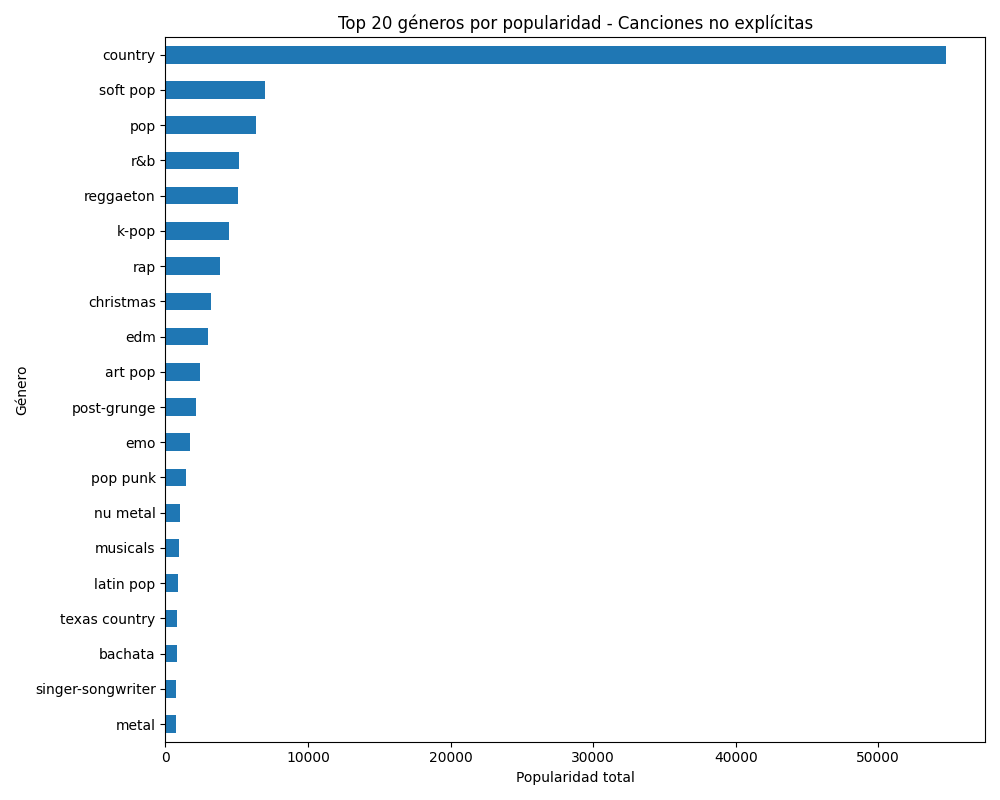
\includegraphics[width=0.7\textwidth]{popular_genres.png}
\end{center}

\end{sectionbox}

\pagebreak

\begin{sectionbox}{Actividad 3: Puntajes por videojuego}

Escriba una función que reciba una tupla con información de puntajes de videojuegos y el nombre de un videojuego, y retorne una tupla con el jugador que obtuvo el mayor puntaje en ese videojuego y el valor de ese puntaje.

La tupla de información contiene tres elementos:
\begin{itemize}
    \item Una matriz donde cada fila representa un videojuego y cada columna representa un jugador
    \item Una lista con los nombres de los videojuegos (en el mismo orden que las filas)
    \item Una lista con los nombres de los jugadores (en el mismo orden que las columnas)
\end{itemize}

Si el videojuego especificado no existe en los datos, la función debe retornar la tupla \texttt{(None, None)}.

\textbf{E.g.:} Si la matriz es \texttt{[[5000, 3200], [1200, 8400]]}, los videojuegos son \texttt{["Tetris", "Pac-Man"]}, los jugadores son \texttt{["María", "Pedro"]}, y se consulta por \texttt{"Pac-Man"}, la función debe retornar \texttt{("Pedro", 8400)} porque 8400 es mayor que 1200.

\end{sectionbox}

\pagebreak

\begin{sectionbox}{Actividad 4: Simulación de ecosistema}

Escriba una función que reciba una matriz cuadrada representando un ecosistema y retorne las coordenadas del primer conejo que huirá. Si ningún conejo huirá, debe retornar \texttt{(None, None)}.

En la matriz, cada posición puede contener:
\begin{itemize}
    \item \texttt{0}: Terreno vacío
    \item \texttt{1}: Conejo (en calma)
    \item \texttt{2}: Zorro (depredador)
\end{itemize}

Un conejo huirá si cumple estas dos condiciones simultáneamente:
\begin{enumerate}
    \item Hay zorros en las posiciones inmediatamente a su izquierda y a su derecha. Si alguna de estas posiciones no existe porque el conejo está en el borde del ecosistema, esta condición no se cumple.
    \item La posición inmediatamente adelante no contiene un zorro. Si la posición adelante no existe porque el conejo está en la primera fila, esta condición sí se cumple.
\end{enumerate}

El recorrido debe realizarse de adelante hacia atrás (de arriba hacia abajo) y de izquierda a derecha.

\textbf{E.g.:} Si hay un conejo en la posición (1,1), hay zorros en (1,0) y (1,2), y la posición (0,1) no contiene un zorro, entonces ese conejo huirá y sus coordenadas deben ser retornadas.

\end{sectionbox}

\pagebreak

\begin{sectionbox}{Entrega}

Entregue un archivo comprimido (ZIP) que contenga:

\begin{enumerate}
    \item \textbf{analisis\_musica.py}: Implementación de las Actividades 1-2
    \item \textbf{matrices.py}: Implementación de las Actividades 3-4
\end{enumerate}

Suba el archivo comprimido a través de Bloque Neón en el laboratorio del Nivel 4 designado como ``N4-L3: Análisis de datos y matrices''.

\end{sectionbox}

\end{document}
